\documentclass[xcolor=pdftex, dvipsnames, table]{beamer}

\RequirePackage[russian]{babel}
\RequirePackage[utf8]{inputenc}
\RequirePackage[TS1,T2A]{fontenc}
\usepackage{float}
\usepackage{amsmath}
\usepackage{listings}

\floatstyle{ruled}
\newfloat{program}{h}{src}
\floatname{program}{Листинг}

\usepackage{beamerthemeBoadilla}

\title{Система учёта и управления электронными налоговыми декларациями.}
\author{Залунин Павел}
\institute {
  БГУИР\\
  ФИТУ
}

\begin{document}

\frame{\titlepage}

\section[Outline]{}
\frame{\tableofcontents}

\section{Введение}
\subsection{Актуальность}
\begin{frame}
  \frametitle{Актуальность}
  \begin{block}{Предпосылки}
    \begin{itemize}
    \itemЗаполнение финансовых документов весьма трудоемкий процесс, включающий в себя операции с большим объемом данных. Данные представляют собой различные аспекты деятельности предприятия, которые так же необходимо учитывать.
    \itemПравила заполнения финансовых документов меняются как минимум раз в финансовый год.
    \itemНа больших предприятиях существует потребность в заполнении большого количества документов, что влечет за собой большие финансовые затраты.
    \end{itemize}
  \end{block}
\end{frame}

\subsection{Налоговая декларация}
\begin{frame}
  \frametitle{Налоговая декларация}
  \begin{block}{Налоговая декларация}
    Документ, содержащий данные о финансовой деятельности предприятия.
  \end{block}
  Существуют различные налоговые формы ( активные доходы, пассивные доходы, налог на $CO^{2}$ и др.)
  \begin{center}
    \includegraphics[width=0.9\textwidth,maxheigth=0.9\textheight]{pics/declaration}
  \end{center}
\end{frame}

\begin{frame}
  \frametitle{Существующие решения}
  Были рассмотрены следующие коммерческие решения:
  \begin{center}
    \small {
      \rowcolors{1}{RoyalBlue!20}{RolalBlue!5}
      \begin{tabular}{|p{2cm}|p{2cm}|p{1.5cm}|p{1.6cm}|p{2.3cm}|}\hline
        \bfseries{Название системы} &
        \bfseries{Тип} &
        \bfseries{ОС} &
        \bfseries{Структура} &
        \bfseries{База Данных}\\
        \hline
        1C Бухгалтерия & Система бухгалтерского учета & Windows, GNU Linux & Standalone, Web & 1CD, Microsoft SQL Server, DBF\\
        \hline
        Галлактика ERP & СПРП\footnote[1]{Система планирования ресурсов предприятия\label{erp}} & Windows  & Standalone  & PervasiveSQL, Microsoft SQL Server, Oracle\\
        \hline
        Парус & СПРП$^{1}$ & Windows & Standalone, Web & Oracle\\
        \hline
        Microsoft Dynamic NAV & СПРП$^{1}$ & Windows & Standalone, Web & Microsoft SQL Server\\
        \hline
      \end{tabular}
    }
  \end{center}
  \\
\end{frame}

\section{Проектирование}
\subsection{Структура системы}
\begin{frame}
  \frametitle{Структура системы}
  \begin{center}
    \includegraphics[width=0.7\textwidth,maxheight=0.8\textheight]{pics/system_struct}
  \end{center}
\end{frame}
\subsection{Требования}
\begin{frame}
  \frametitle{Требования, предъявленные к системе}
  \begin{itemize}
    \item Web интерфейс;
    \item использование реляционной БД;
    \item возможность добавление новых деклараций и изменения существующих, необходимо предоставить простой способ для достижения этой цели;
    \itemредактирование декларации должно осуществляться интерактивно, без перезагрузки страницы;
    \itemна декларации может присутствовать три типа ячеек: a) формула b) интервальная c) пользовательская;
    \itemтребуется предоставить возможность задания произвольного значения для ячейки, которая считается по каким-либо правилам.
  \end{itemize}
\end{frame}

\begin{frame}
  \frametitle{Проектирование системы}
  \begin{enumerate}
    \item Выделение объектов: диаграмма \textbf{<<Сущность-связь>>}.
    \item Выделение вариантов использования: диаграммы \textbf{вариантов использования}.
    \item Анализ вариантов использования: \textbf{диаграммы последовательности}.
    \item Детализация объектов: \textbf{выделение} новых \textbf{объектов}, \textbf{алгоримтов} подсчёта ячеек, \textbf{грамматика} языка для описание формул, \textbf{диаграмма активности}.
    \item Представление \textbf{структуры декларации} на языке XML.
    \item Логическая \textbf{модель данных}.
  \end{enumerate}
\end{frame}

\section{Реализация}
\begin{frame}
  \frametitle{Реализация системы}
  \begin{enumerate}
    \item Выбор инструментальных средств разработки
    \item Реализация классов-сущностей.
    \item Реализация подсистемы управления.
    \item Реализация подсистемы управления декларацией.
    \item Реализация подсистемы хранения.
    \item Реализация подсистемы отображения декларации.
    \item Реализация подсистемы вычисления значения выражения.
    \item Тестирование системы.
  \end{enumerate}
\end{frame}
\begin{frame}
  \frametitle{Инструментальные средства}
  \begin{itemize}
    \item Язык программирования Java.
    \item Интегрированная среда разработки Eclipse.
    \item Набор библиотек Spring (использовались модули Spring MVC, Spring IoC).
    \item Библиотека Hibernate.
    \item Библиотека JUnit.
    \item Сервер приложений Apache Tomcat.
    \item Технология Java Server Pages.
    \item Язык сценариев JavaScript.
    \item Технология AJAX.
    \item Средство сборки приложений Maven.
  \end{itemize}
\end{frame}
\begin{frame}
  \frametitle{Реализация подсистемы управления}
  \begin{columns}
    \begin{column}{0.6\textwidth}
      \begin{center}
        \begin{figure}
          \includegraphics[scale=0.23]{pics/springmvc}
          \caption{Обработка запроса Spring MVC}
          \label{pic:springmvc}
        \end{figure}
      \end{center}
    \end{column}
    \begin{column}{0.5\textwidth}
      \begin{itemize}
        \item CompanyController
        \item TaxKitController
        \item TaxKitEditController
        \item LedgerController
        \item ReportStateController
        \item ReportController
      \end{itemize}
    \end{column}
  \end{columns}
\end{frame}

\begin{frame}
  \frametitle{Реализация подсистемы хранения}
  Объектно-реляционное отображение. Библиотека Hibernate.
  \begin{center}
    \includegraphics[width=0.9\textwidth]{pics/orm}
  \end{center}
\end{frame}

\begin{frame}
  \frametitle{Интерфейс пользователя. Редактирование декларации.}
  \begin{center}
    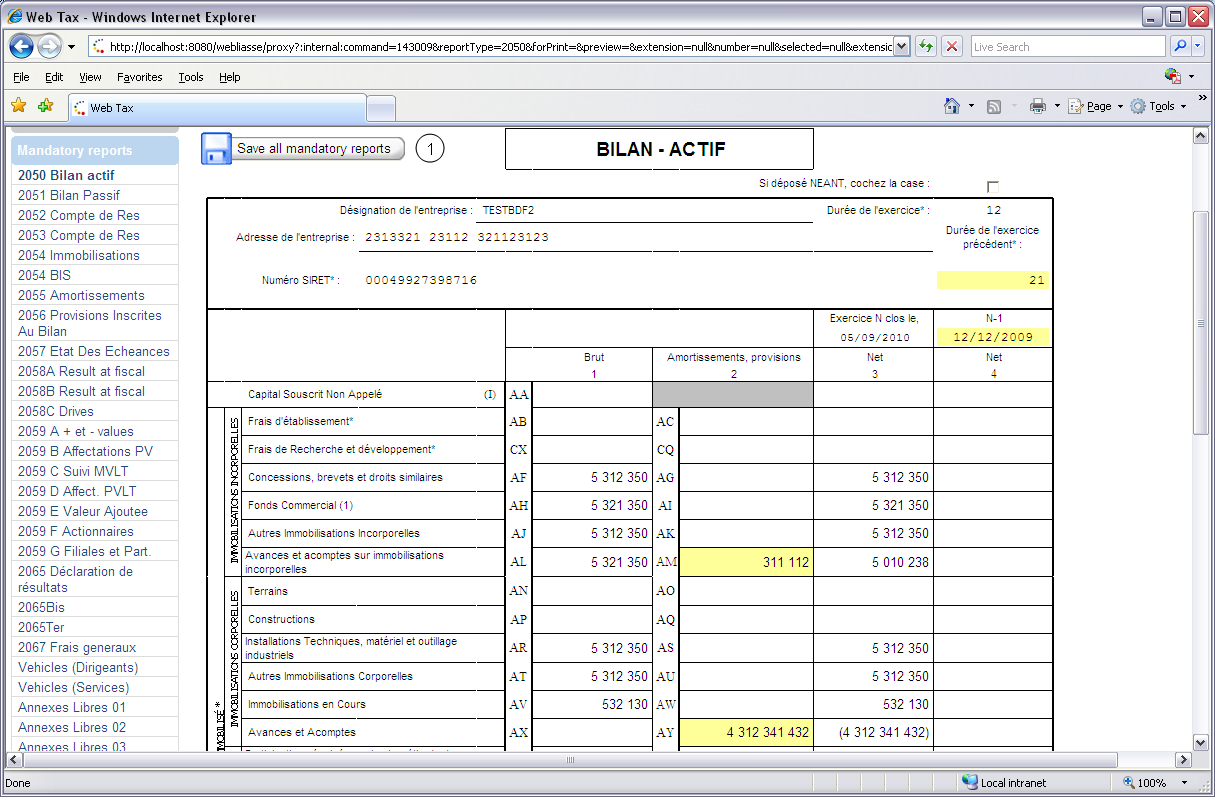
\includegraphics[width=0.9\textwidth]{pics/src_reportnice}
  \end{center}
\end{frame}


\section{Тестирование}
\subsection{Модульные тесты}
\begin{frame}
  \frametitle{Модульные тесты}
  В целях тестирования кода и контроля качества во время разработки были реализованы модульные тесты.
  Результат выполнения:
  \begin{center}
    \small {
      \rowcolors{1}{RoyalBlue!20}{RolalBlue!5}
      \begin{tabular}{|m{6cm}|m{2cm}|m{2cm}|} \hline
        \textbf{Класс} &
        \textbf{Кол-во тестов} &
        \textbf{Успешные тесты} \\ \hline
        ReportFactoryImplTest & 1 & 100\% \\ \hline
        ReportManagerTest & 3 & 100\% \\ \hline
        ReportCrossInterpreterTest & 1 & 100\% \\ \hline
        ReportInterpreterTest & 1 & 100\% \\ \hline
        XMLReportLoaderTest & 1 & 100\% \\ \hline
        XMLCellLoaderTest & 2 & 100\% \\ \hline
        XMLFileReaderTest & 3 & 100\% \\ \hline
        AccountsInterpreterTest & 1 & 100\% \\ \hline
        ReflectionAssemblerTest & 1 & 100\% \\ \hline
        ExpressionParserTest & 2 & 100\% \\ \hline
        CompanyControllerTest & 2 & 100\% \\ \hline
        ReportStateControllerTest & 5 & 100\%  \\ \hline
        ReportsServiceImplTest & 1 & 100\%  \\ \hline
        TaxKitReportStateDAOImplTest & 1 & 100\%  \\ \hline
      \end{tabular}
    }
  \end{center}
\end{frame}

\section{Заключение}
\begin{frame}
  \frametitle{Заключение}
  Для выполнения дипломного проекта были решены следующие задачи:
  \begin{itemize}
    \item Анализ предметной области
    \item Проектирование системы
    \item Реализация системы
    \item Тестирование системы
    \item Выделение мер, обеспечивающих комфортные условия труда разработчикам систем документооборота
    \item Произведено технико-экономическое обснование эффективности внедрения программного продукта
  \end{itemize}
\end{frame}
\begin{frame}
  \begin{center}
    \begin{huge}
      Спасибо за внимание.
    \end{huge}

    Вопросы, ответы.
  \end{center}
\end{frame}


\end{document}
